\myChapter{Sleep event detection}
% \begin{flushright}{\slshape
% 		It's a magical world, Hobbes, ol' buddy\ldots\\
% 		\ldots Let's go exploring!}\\ \medskip
% 		--- Calvin\\Calvin and Hobbes, by\defcitealias{Watterson1996}{Bill Watterson}\citetalias{Watterson1996} \citep{Watterson1996}
% \end{flushright}
\vspace{6cm}

This chapter presents the methods developed for detection of sleep events.
Specifically, the \ac{MSED} algorithm originally published in~\cite{Olesen2019} for arousal and limb movement detection is presented first in~\cref{sec:paperiv}, which is then followed by the updated version. A method for improving single-\ac{EEG} arousal detection is also included in~\cref{sec:paperv}. The chapter will conclude with a summary and discussion of the main findings of the individual research items in~\cref{sec:eventdetection-summary}.

Parts of this chapter have been modified from the following original publications:
% \paragraph{\Cref{sec:paperiv}} has been modified from\newline \fullcite{Olesen2019}\footnote{\textcopyright 2019 IEEE}
% \paragraph{\Cref{sec:paperv}} has been modified from\newline \fullcite{Olesen2020b} (\textit{submitted})
\begin{itemize}
    \item \fullcite{Olesen2019}\footnote{\textcopyright 2019 IEEE}
    \item \fullcite{Olesen2020b} (\textit{submitted})
\end{itemize}


\section{Research background}

As described in~\cref{chap:clinical-background}, correct diagnosis of sleep disorders is predicated on precise scoring of sleep stages as well as accurate scoring of these discrete sleep events. 
However, the current gold standard of manual analysis by experienced technicians is inherently biased and inconsistent and several studies have shown low inter-rater reliability on both the scoring of sleep stages~\cite{Norman2000,Rosenberg2013,Younes2016}, arousals~\cite{Bonnet2007}, and respiratory events~\cite{Rosenberg2014}. 
Furthermore, manual analysis of \acsp{PSG} is time-consuming and prone to scorer fatigue. 
Thus, there is a need for efficient systems that provide deterministic and reliable scorings of sleep studies.

Several recent studies have already explored automatic classification of sleep stages in large cohorts with good results~\cite{Olesen2018,Stephansen2018,Chambon2018a,Biswal2018, Phan2018}, however, the reliable and consistent detection and classification of discrete PSG events in large cohorts remain largely unexplored. 

Recent studies on certain micro-events in sleep have indicated that sleep spindles and K-complexes can be reliably detected and annotated with start time and duration using deep learning methods~\cite{Chambon2018b,Chambon2019}. 
Specifically, these studies proposed a single-shot event detection algorithm, that parallels the YOLO and SSD algorithms used for object detection in 2D images~\cite{Redmon2016,Liu2016}, however, they were limited in scope by detecting events only at the \ac{EEG} level, and did not explicitly take advantage of the temporal connection of the detected events. 
Additionally, experiments were carried out on a small-scale database~\cite{Chambon2018b}. 

Designing reliable and robust systems for automated sleep analysis based on machine learning algorithms often require multiple heterogenous data sources of sufficient size.
However, due to differences in clinical practice, very few datasets in sleep science are standardized with regards to recording setups despite guidelines from the \ac{AASM}.

In these cases, we end up with a \textit{channel mismatch problem}, in which the overlap between our source and target domains is small, and the domains are possibly disjointed. 
Recent studies have investigated the use of deep transfer learning to solve the channel mismatch problem when training and testing sleep stage classification models~\cite{Phan2019, Phan2019c}.
The authors found that using a fine-tuning strategy significantly improved the performance of sleep stage scoring models when trained on various combinations of \ac{EEG} and \ac{EOG} channels.

\subsection{Research questions}

% Research papers
\section{Paper IV: Towards a flexible deep learning method for automatic detection of clinically relevant multi-modal events in the polysomnogram}\label{sec:paperiv}
\sectionmark{Olesen, Chambon, Thorey, Jennum, Mignot, \& Sorensen, 2019}
% \sectionmark{{\protect\citeauthor{Olesen2019}}}

\begin{tcolorbox}[colframe=white]
\paragraph{Abstract: } 
Much attention has been given to automatic sleep staging algorithms in past years, but the detection of discrete events in sleep studies is also crucial for precise characterization of sleep patterns and possible diagnosis of sleep disorders. 
We propose here a deep learning model for automatic detection and annotation of arousals and leg movements. 
Both of these are commonly seen during normal sleep, while an excessive amount of either is linked to disrupted sleep patterns, excessive daytime sleepiness impacting quality of life, and various sleep disorders. 
Our model was trained on 1485 subjects and tested on 1000 separate recordings of sleep. 
We tested two different experimental setups and found optimal arousal detection was attained by including a recurrent neural network module in our default model with a dynamic default event window (F1 = 0.75), while optimal leg movement detection was attained using a static event window (F1 = 0.65). 
Our work show promise while still allowing for improvements. 
Specifically, future research will explore the proposed model as a general-purpose sleep analysis model.
\end{tcolorbox}

\subsection{Materials \& Methods}

\subsubsection{MrOS Sleep Study}
The MrOS Sleep Study is a part of the larger Osteoporotic Fractures in Men Study with the objective of researching the links between sleep disorders, fractures, cardiovascular disease and mortality in older males (\num{>65} years)~\cite{Blank2005,Orwoll2005,Blackwell2011}. 
Between 2003 and 2005, 3135 of the original 5994 participants were recruited to undergo full-night \ac{PSG} recording at six centers in the US at two separate visits (visit 1 and visit 2) with following 3 to 5-day actigraphy studies at home. 
The resulting \ac{PSG} studies were subsequently scored by experienced sleep technicians for standard sleep variables including sleep stages, leg movements, arousals, and respiratory events.

\subsubsection{Included events and signals}
In this study, we only considered the detection of two \ac{PSG} events: arousals and leg movements. 
These events are characterized by a start time and a duration, which we extracted from 2907 \ac{PSG} studies from visit 1 available from the National Sleep Research Resource repository~\cite{Dean2016,Zhang2018}. 
From each \ac{PSG} study, we extracted left and right central \ac{EEG}, left and right \ac{EOG}, chin \ac{EMG}, and \ac{EMG} from the left and right anterior tibialis. 
\Ac{EEG} and \ac{EOG} channels were referenced to the contralateral mastoid process, while a leg \ac{EMG} channel was synthesized by referencing left to right. 
Any \ac{PSG} without the full set of channels or without any event scoring was eliminated from further analysis.

\subsubsection{Subset demographics and partitioning}
In total, 2650 out of the 2907 \acp{PSG} available from visit 1 were included in this study. 
These were partitioned into \train, \eval, and \test sets containing 1485, 165, and 1000 studies, respectively. 
A subset of key demographic and \ac{PSG} variables are presented in~\cref{tab:paperiv-demographics}.

\begin{table}
  \small
  \centering
  \sisetup{separate-uncertainty}
  \begin{threeparttable}
%   \begin{adjustwidth*}{}{-\marginparwidth-\marginparsep}
  \caption[\acs{MrOS} data demographics]{\acs{MrOS} data demographics.}
  \label{tab:paperiv-demographics}
%   \footnotesize
%   \renewcommand{\arraystretch}{1.3}
  \setlength\tabcolsep{5pt}
  \begin{tabular}{lSSSS}
    \toprule
                                           & \train & \eval & \test & \textit{p}-value \\
    \midrule
    \textit{N}                                      & \num{1485} & \num{165}  & \num{1000} & \\
    Age, years                             & \num{76.4 \pm 5.5} & \num{76.6 \pm 4.9} & \num{76.4 \pm 5.6 } & \num{0.631} \\
    \acs{BMI}, \si{\kilogram\per\square\second} & \num{27.2 \pm 3.8 } & \num{ 27.2 \pm 3.4 } & \num{27.1 \pm 3.7 } & \num{0.879} \\
    \acs{AHI}, \si{\per\hour}                   & \num{12.8 \pm 12.9 } & \num{ 10.6 \pm 11.8 } & \num{11.9 \pm 12.8 } & {\bfseries \num{0.029}} \\
    \acs{ArI}, \si{\per\hour}                    & \num{23.6 \pm 11.5 } & \num{ 24.1 \pm 12.2 } & \num{23.4 \pm 11.8 } & \num{0.607} \\
    \acs{PLMI}, \si{\per\hour}                  & \num{34.8 \pm 37.0 } & \num{ 37.8 \pm 38.9 } & \num{37.3 \pm 38.0 } & \num{0.204} \\
    \bottomrule
  \end{tabular}
  \begin{tablenotes}
  \item Continuous variables were tested for significance with Mann-Whitney U-tests.
  Significant \textit{p}-values at $\alpha=\num{0.05}$ are shown in bold. %
  \describe{BMI}; %
  \describe{AHI}; %
  \describe{ArI}; %
  \describe{PLMI}.
  \end{tablenotes}
  \end{threeparttable}
  
%   \end{adjustwidth*}
\end{table}

\subsubsection{Signal preprocessing}
All signals were resampled to \(f_s = \SI{128}{\hertz}\) using poly-phase filtering
% \graffito{This is a piece of text in your margin} 
with a Kaiser window ($\beta = \num{5.0}$) before subsequent filtering according to \ac{AASM} criteria~\cite{Berry2020}.
Briefly, \ac{EEG} and \ac{EOG} channels were subjected to a \nth{4} order digital Butterworth band-pass filter with a \SIrange{0.3}{35}{\hertz} passband, while chin and leg \ac{EMG} channels were filtered with a \nth{4} order digital Butterworth high-pass filter with a \SI{10}{\hertz} cutoff frequency.
All filters were implemented using zero-phase filtering\graffito{The zero-phase filtering procedure filters a signal in the forward direction, and then in the reverse direction, while matching the initial conditions of the filter in the reverse direction.}.
Lastly, each channel was normalized by subtracting the channel mean and dividing by the channel standard deviation across the entire night.

\subsubsection{Detection model overview}
In brief, the proposed model receives as input a tensor $\mathbf{x}\in \real{C \times T}$ containing $C$ channels of data in a segment of $T$ samples, along with a set of events $\lbrace \varepsilon_{i} \in \real{2} \mid \varepsilon_i = \left( \varrho_{i}, \delta_{i} \right),\, i\in \llbracket N_{\mathbf{x}} \rrbracket \rbrace$, were $N_{\mathbf{x}}$ is the number of events in the associated time segment and $\left(\varrho_{i},\delta_{i}\right)$ are the start time and duration of event $\varepsilon_i$.
The objective of the deep learning model $f$ is then to infer $\lbrace \varepsilon_{i} \rbrace$ given $\mathbf{x}$.
To do this, a set of default events $\lbrace \varepsilon_{j}^{d} \in \real2 \mid j\in\llbracket N_{d} \rrbracket,\, N_{d} = T/\tau \rbrace$ is generated over the segment of $T$ samples, where $\tau$ is the size of each default event window in samples.
The model outputs probabilities for $K$ classes including the default, non-event class for each default event window.
The probability for a given class $k$ in the default event window $\varepsilon_j^d$ must be greater than a classification threshold $\theta_{\mathrm{clf}}$.
In order to select among many possible candidates of predicted events, all predicted events of class $k$ over the possible events in $N_d$ is subjected to non-maximum suppression using the \ac{IoU}\graffito{The \acf{IoU} is also known as the Jaccard index.} as in~\cite{Redmon2016a,Redmon2016b}.
A high-level schematic of the detection model is shown in~\cref{fig:paperiv-schematic}.

\begin{figure}
\begin{adjustwidth*}{}{-\marginparwidth-\marginparsep}
\centering
    % 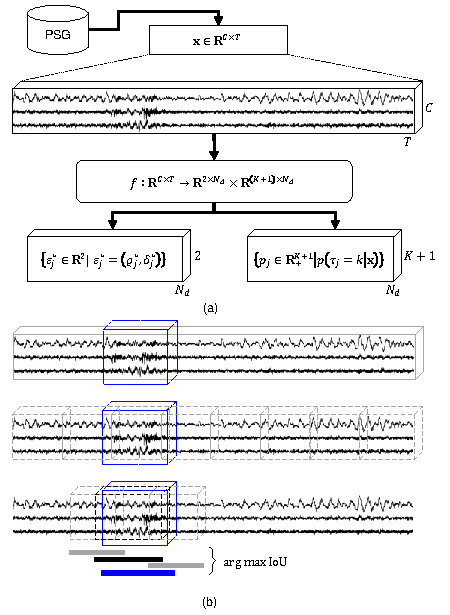
\includegraphics[width=\columnwidth+\marginparwidth+\marginparsep]{figures/paper-iv/embc19-psg_event_detection-fig1-ppt.pdf}
    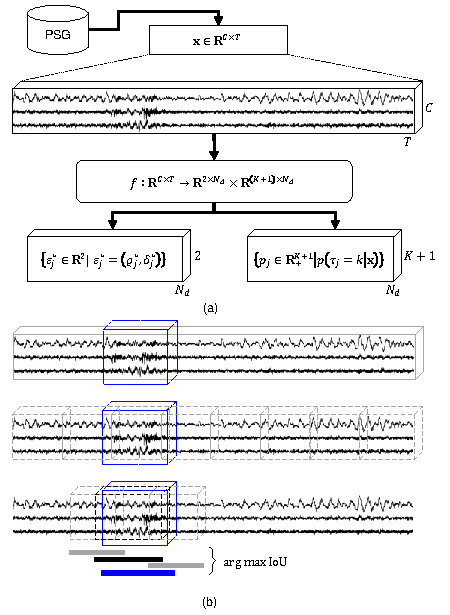
\includegraphics[width=\linewidth]{figures/paper-iv/embc19-psg_event_detection-fig1-ppt.pdf}
    \caption[Event detection schematic]{Schematic of proposed event detection procedure. \textbf{(a)} Input data $\mathbf{x}$ is fed to the model $f$, which outputs predictions for event classes and localizations for each default event in $\varepsilon^{d}$. \textbf{(b)} The IoU for each predicted $\varepsilon^{*}_{j}$ is then calculated with respect to the true event $\varepsilon_{i}$ and non-maximum suppression is applied to match up true events and predictions. In the current case, the predicted event marked in black has the highest IoU with the true event in blue. For more information, see~\cite{Chambon2019,Chambon2018b,Liu2016}.}
    \label{fig:paperiv-schematic}
\end{adjustwidth*}
\end{figure}

\begin{table}
\small
\begin{adjustwidth*}{}{-\marginparwidth-\marginparsep}
\begin{threeparttable}
% \centering
\caption[Event detection network architecture]{Event detection network architecture.}
\label{tab:paperiv-network}
{\footnotesize
\begin{tabular}{@{}lccccccl@{}} \toprule
\textbf{Module}                                                     & \textbf{Input dim.}                                 & \textbf{Output dim.}                                    & \textbf{Type}           & \textbf{Kernel} & \textbf{Filters}                  & \textbf{Stride}      & \textbf{Activation} \\ \midrule
$\phi_{C}$                                                 & $\left(C, T\right)$                        & $\left(C, T\right)$                            & \oned conv & $C$         & $C$                          & 1           & linear \\ \midrule
\multirow[t]{3}{*}{$\phi_{T,\mathrm{init}}$}                  & $\left(C, T\right)$                        & $\left(8, T\right)$                            & \oned conv & $3$         & 8                            & $1$         & -- \\
& $\left(8, T\right)$                        & $\left(8, T\right)$                            & batch norm.    & --          & 8                            & --          & \acs{ReLU} \\
& $\left(8, T\right)$                        & $\left(8, \sfrac{T}{2}\right)$                 & \oned maxpool  & $2$         & --                           & $2$         & -- \\
\multirow[t]{3}{*}{$\phi_{T,n}$} & $\left(2^{n+1}, \sfrac{T}{2^{n-1}}\right)$ & $\left(2^{n+2}, \sfrac{T}{2^{n-1}}\right)$     & \oned conv & $3$         & $2^{n+2}$                    & $1$         & -- \\
& $\left(2^{n+2}, \sfrac{T}{2^{n-1}}\right)$ & $\left(2^{n+2}, \sfrac{T}{2^{n-1}}\right)$     & batch norm.    & --          & $2^{n+2}$                    & --          & \acs{ReLU} \\
& $\left(2^{n+2}, \sfrac{T}{2^{n-1}}\right)$ & $\left(2^{n+2}, \sfrac{T}{2^{n}}\right)$       & \oned maxpool  & $2$         & --                           & $2$         & -- \\ 
\rowcolor{lightlightgray} $\phi_{R}$ & $(\tilde{C}, \tilde{T})$ & $(2\times \tilde{C}, \tilde{T})$ & \acs{bGRU} & $\tilde{C}$ & -- & -- & -- \\ \midrule
$\psi_{\mathrm{clf}}$                                      & $(\tilde{C}, \tilde{T})$                   & $\left( K N_{d}, 1 \right)$ & \oned conv & $\tilde{T}$ & $K N_{d}$ & $\tilde{T}$ & softmax over $K$ filters \\
$\psi_{\mathrm{loc}}$                                      & $(\tilde{C}, \tilde{T})$                   & $\left( 2 N_{d}, 1 \right)$                    & \oned conv & $\tilde{T}$ & $2 N$                        & $\tilde{T}$ & linear \\ \bottomrule
\end{tabular}}
\begin{tablenotes}
\item $\phi_C$, linear mixing module; $\phi_{T}$, temporal feature extraction module; $\phi_{R}$, recurrent neural network module; $\psi_{\mathrm{clf}}$, event classification module; $\psi_{\mathrm{loc}}$, event localization module; $C$, number of input channels; $T$, number of samples in segments; $\tilde{C}=2^{2+n_{\max}}$, number of output channels; $K$, number of event classes; $N_{d}$, number of default events in segment; $\tilde{T}=\sfrac{T}{2^{n_{\max}}}$, reduced temporal dimension; \acs{bGRU}, bidirectional gated recurrent unit; \acs{ReLU}, rectified linear unit.
\end{tablenotes}
\end{threeparttable}
\end{adjustwidth*}
\end{table}

\subsubsection{Network architecture}
The architecture for the proposed \ac{PSG} event detection model closely follows the event detection algorithms described in~\cite{Chambon2018b,Chambon2019}, albeit with some specific changes.
An overview of the proposed network in the model $f$ is provided in~\cref{tab:paperiv-network}.
Briefly, the model comprises three modules:
\begin{enumerate}
\item a channel mixing module $\phi_{C} : \real{C \times T} \to \real{C \times T}$;
\item a feature extraction module $\phi_{T} : \real{C \times T} \to \real{\tilde{C} \times \tilde{T}}$;
\item and an event detection module $\psi$,
\end{enumerate}
the latter contains two submodules performing event classification $\psi_{\mathrm{clf}} : \real{\tilde{C} \times \tilde{T}} \to \real{(K+1)\times N_{d}} $ and event localization $\psi_{\mathrm{loc}} : \real{\tilde{C} \times \tilde{T}} \to \real{2 \times N_{d}}$, respectively.
$\phi_{\mathrm{clf}}$ outputs the probability of the default, non-event class and $K$ event classes, while $\phi_{\mathrm{loc}}$ predicts a start time and a duration of all predicted events relative to a specific default event window.
The channel mixing module $\phi_{C}$ receives a segment of input data $x \in \real{C \times T}$, where $C$ is the number of input channels and $T$ is the number of time samples in the given segment, and subsequently performs linear channel mixing using \oned~convolutions to synthesize $C$ new channels. 
Following $\phi_{C}$, the feature extraction module $\phi_{T}$ consists of $n_{\max}$ blocks with the first block $\phi_{T,1} : \real{C \times T} \to \real{8 \times \sfrac{T}{2}}$ and the $n$th block $\phi_{T,n} : \real{2^{n+1} \times \sfrac{T}{2^{n-1}}} \to \real{2^{k+2} \times \sfrac{T}{2^{n}}}$.
All $n_{\max}$ blocks implement $\phi_{T,n}$ using \oned~convolution layers followed by batch normalization of the feature maps, rectified linear unit activation, and final \oned maximum pooling layers across the temporal dimension.
Kernel sizes and strides for convolution and max. pool. layers in $\phi_{T}$ were set to 3 and 1, and 2 and 2, respectively, while the number of feature maps in $\phi_{T,n}$ was set to $2^{n+2}$.
The event classification submodule $\psi_{\mathrm{clf}}$ is implemented a \oned convolution layer across the entire data volume using $(K+1)N_{d}$ feature maps of size and stride $\tilde{T} = T/2^{n_{\max}}$, where $K \in \mathbf{N}$ is the number of event classes to be detected and $N_{d} \in \mathbf{N}$ is the number of default event windows.
The event localization submodule $\psi_{\mathrm{loc}}$ is likewise implemented using a \oned convolution layer across the entire data volume.

\subsubsection{Data and event sampling}
The proposed network requires an input tensor $x \in \real{C \times T}$ containing \ac{PSG} data in the time segment of size $T$ as well as information about the associated events in the segment.
Since the total number of segments in a standard \ac{PSG} without any event data by far outnumbers the number of segments with event data, we implemented a random sampling of non-event and event classes with the sampling probability of class $k$ inversely proportional to the number of classes, such that $p_k = \frac{1}{K+1},\,k=\left[0\,..\,K \right]$, where $k=0$ is the default (non-event) class.
At training step $t$, we thus sample a class $k$ and afterwards randomly sample a single class $k$ event $\varepsilon_{k}$ between all class $k$ events.
Finally, we extract a segment of \ac{PSG} data of size $C \times T$ with start of segment in the interval $\left[ \bar{\varepsilon}_{k} - T, \bar{\varepsilon}_{k} + T \right]$, where $\bar{\varepsilon}_{k}$ is the sample midpoint of $\varepsilon_{k}$.
This ensures that each $\mathbf{x}$ overlaps 50\% with at least one associated event.

\subsubsection{Optimization of network parameters}
The network parameters were optimized using mini-batch stochastic gradient descent with initial learning rate of \num[retain-unity-mantissa = false]{1e-3} and a momentum of \num{0.9}. 
Mini-batches were balanced with respect to the detected classes. 
The optimization of the network was performed with respect to the same loss function described in~\cite{Chambon2018b,Chambon2019}\graffito{We used a worst negative mining approach with a positive/negative sample ratio of 3.}, and the network was trained until convergence determined by no decrease in the loss on the \eval set over 10 epochs of \train data. 
We also employed learning rate decay with a factor of 2 every 5 epochs of non-decreasing \eval loss.

\subsubsection{Experimental setups}
In this study, we examined two different experimental setups:
\paragraph{Experiment A} First, we investigated the differences in predictive performance using a static vs. a dynamic default event window size. 
This was realized by running six separate training runs with $\tau \in \lbrace \numlist[list-final-separator={, }]{3;5;10;15;20;30} \rbrace \times f_{s}$, as well as a single training run where $f$ was evaluated for all $\tau$ in $\lbrace \numlist[list-final-separator={, }]{3;5;10;15;20;30} \rbrace \times f_{s}$. 
The best performing model was determined by evaluating F1 score on the \eval set for both \ac{LM} and \ac{Ar} detection. 
\paragraph{Experiment B} Second, we tested a network where we added a recurrent processing block $\phi_{R}$ after the feature extraction block $\phi_{T}$ as shown in grey in~\cref{tab:paperiv-network}. 
We considered a single \ac{bGRU} layer with $\tilde{C}$ units. 
Predictions were evaluated across multiple time-scales $\tau \in \lbrace \numlist[list-final-separator={, }]{3;5;10;15} \rbrace \times f_{s}$.

All experiments were implemented in PyTorch 1.0~\cite{Paszke2017,Paszke2019}.

\subsubsection{Performance metrics}
All models were evaluated on the \eval and \test sets using precision (Pr), recall (Re), and F1 scores (F1):
\begin{align}
    \mathrm{Pr} &= \frac{\mathrm{TP}}{\mathrm{TP} + \mathrm{FP}}, \quad \mathrm{Re} = \frac{\mathrm{TP}}{\mathrm{TP} + \mathrm{FN}} \\
    \mathrm{F1} &= 2 \frac{\mathrm{Pr} * \mathrm{Re}}{\mathrm{Pr} + \mathrm{Re}} = \frac{2\mathrm{TP}}{2\mathrm{TP} + \mathrm{FP} + \mathrm{FN}},
\end{align}
where TP, FP, and FN, are the number of true positives, false positives and false negatives, respectively.

% \subsubsection{Statistical analysis}
% Demographic and polysomnographic variables were tested for subset differences with Kruskall-Wallis H-test for independent samples.

\subsection{Results and discussion}
% \newcommand{\fullwidth}{-\marginparwidth-\marginparsep}
\begin{figure}
    % \centering
    \begin{adjustwidth*}{}{-\marginparwidth-\marginparsep}
    \myfloatalign   
    \subfloat[]
    {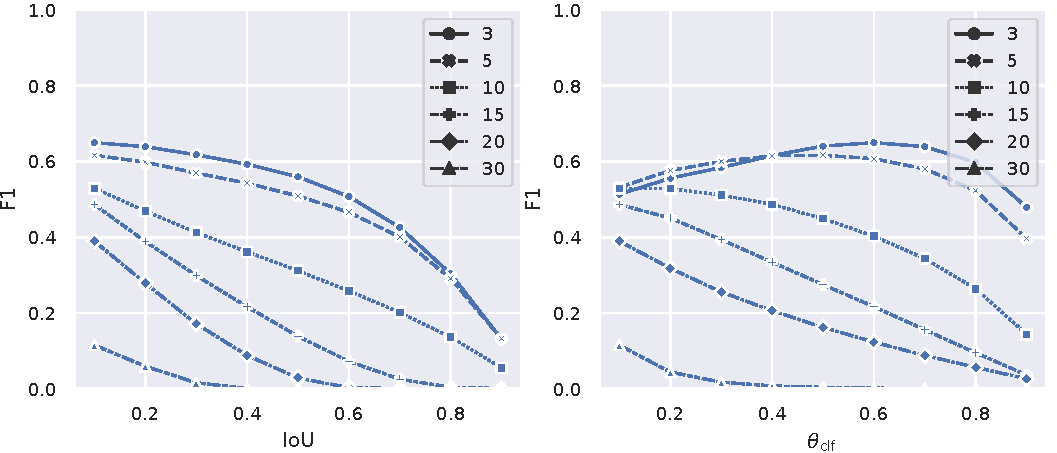
\includegraphics[width=\textwidth]{figures/paper-iv/embc19-mros-limb-default_durations.pdf}\label{fig:paperiv-lm_static}}  \\
    \subfloat[]
    {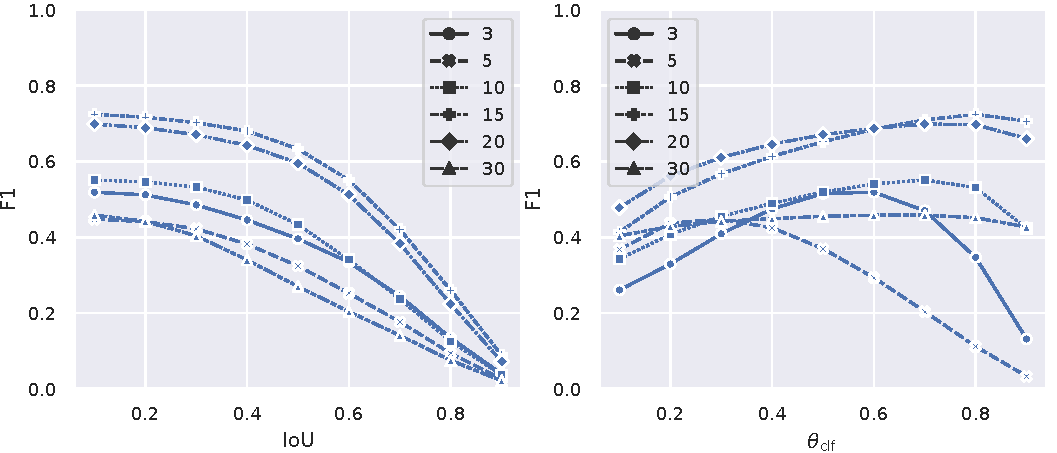
\includegraphics[width=\textwidth]{figures/paper-iv/embc19-arousal-limb-default_durations.pdf}\label{fig:paperiv-ar_static}} \\
    \subfloat[]
    {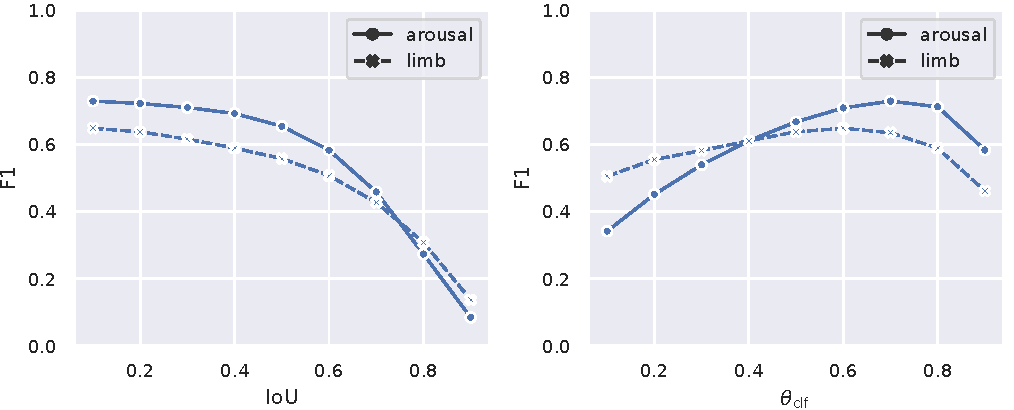
\includegraphics[width=\textwidth]{figures/paper-iv/embc19-mros-arousal_limb-all_durations.pdf}\label{fig:paperiv-ar_lm_dynamic}}
    \caption[Experiment A results]{Experiment A: Optimizing \ac{IoU} and $\theta_{\mathrm{clf}}$ in static models on the \eval set by varying default event window size in seconds in $\lbrace \numlist[list-final-separator={, }]{3;5;10;15;20;30} \rbrace$ \textbf{(a)}-\textbf{(b)}. Left panels show the \ac{IoU} vs. F1 score, while right panels show classification threshold $\theta_{\mathrm{clf}}$ against F1 score. \textbf{(a)} \ac{LM} model. Here, the model performs best for $\mathrm{IoU}=\num{0.1}$ and $\theta_{\mathrm{clf}} = \num{0.6}$ using a window size of $\tau=\SI{3}{\second}\times f_{s}$. \textbf{(b)} \ac{Ar} model. Here, the model performs best for $\ac{IoU}=\num{0.1}$ and $\theta_{\mathrm{clf}} = \num{0.8}$ using a window size of $\tau=\SI{15}{\second} \times f_{s}$. \textbf{(c)} Dynamic models show optimal performance for $\ac{IoU}=\num{0.1}$ and $\theta_{\mathrm{clf}}=\num{0.7}$ and $\theta_{\mathrm{clf}}=\num{0.6}$ for \ac{Ar} and \ac{LM} detection, respectively.}
    \label{fig:paperiv-experiment_a}
    \end{adjustwidth*}
\end{figure}

Shown in~\cref{fig:paperiv-lm_static,fig:paperiv-ar_static} are the F1 scores as a function of \ac{IoU} and the classification threshold $\theta_{\mathrm{clf}}$ for both the \ac{LM} and \ac{Ar} detection models. 
It is apparent that both models perform best with a minimum overlap ($\ac{IoU} = \num{0.1}$) with their respective annotated events, and do not benefit from increasing the overlap. 
This might be caused by the annotated events being imprecise and not by issues with the model itself. 
For example, it is not uncommon to only mark the beginning of an event in standard sleep scoring software, as the duration will automatically be annotated by a default length. \graffito{\SI{3}{\second} for \acp{Ar}, and \SI{0.5}{\second} for \ac{LM} are the minimum durations as defined by \ac{AASM}~\cite{Berry2020}}. 
Future studies will be able to confirm this by either collecting a precisely annotated cohort, or by investigating the average start time and duration discrepancies between annotated and predicted events. 

It is also apparent from~\cref{fig:paperiv-lm_static,fig:paperiv-ar_static} that both detection models benefit from imposing a strict classification threshold. 
Specifically, \ac{LM} detection performance as measured by F1 was highest with $\theta_{\mathrm{clf}} = \num{0.6}$, while maximum \ac{Ar} detection performance was attained with an even higher $\theta_{\mathrm{clf}}$ of \num{0.8}.

By allowing for multiple time-scales in the dynamic models, shown in~\cref{fig:paperiv-ar_lm_dynamic}, we hypothesized that dynamic default event windows would allow for more flexibility and thus better predictive performance. However, we observed no significant differences between the optimal static window and the dynamic window model.

Shown in~\cref{fig:paperiv-experiment_b} are the performance curves for the \ac{RNN} (bidirectional GRU) version of the proposed model for each of the two event detection tasks. 
While the optimal \ac{IoU} and $\theta_{\mathrm{clf}}$ points are unchanged from the static/dynamic models presented in~\cref{fig:paperiv-experiment_a}, the optimal F1 value for \ac{Ar} detection is increased by incorporating temporal dependencies in the model. 
The reverse is true for \ac{LM} detection, which saw a slight decrease in predictive performance caused by lower precision\graffito{See~\cref{tab:paperiv-test_results}}. 
Future work should consider optimizing predictive performance by investigating the effects of varying the number of \ac{bGRU} layers and the number of hidden units in $\phi_{R}$, since this was not performed here.

Application of the optimal models on the \test data is shown in~\cref{tab:paperiv-test_results}. 
With the given architecture of $f$ and the given labels and input data in \train, \ac{LM} detection was maximal for the model with a static/dynamic window, while adding a recurrent module only positively impacted \ac{Ar} prediction. 
Precision and recall decreased for \ac{LM} detection when adding $\phi_{R}$, while precision increased and recall decreased for \ac{Ar} detection. 
An example visualization of the joint distribution of F1 scores obtained from the dynamic model applied to the \test data is shown in~\cref{fig:paperiv-test_distribution}. 
While some outliers are readily observable, especially for \ac{LM} detection, the majority of subject F1 scores follows an approximate bivariate normal distribution.

\begin{figure}
    \centering
    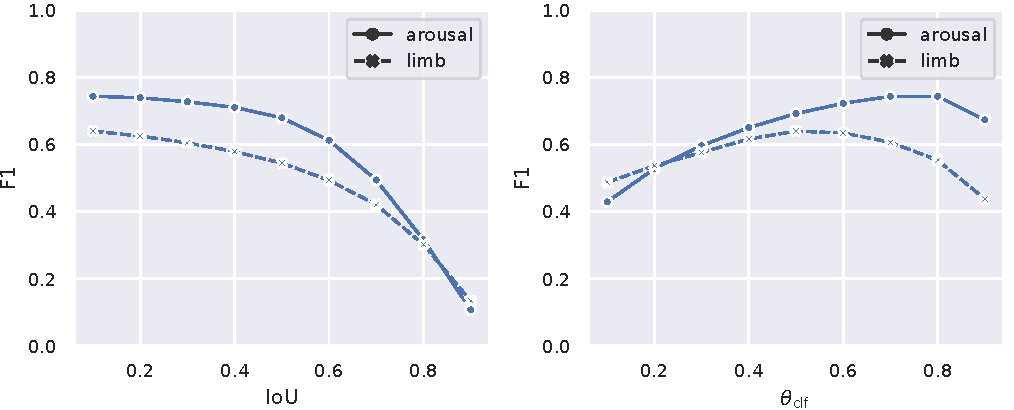
\includegraphics[width=\columnwidth]{figures/paper-iv/embc19-mros-arousal_limb-all_durations_rnn.pdf}
    \caption[Experiment B results]{Experiment B. F1 performance on the \eval set as a function of \ac{IoU} and $\theta_{\mathrm{clf}}$ for \ac{Ar} and \ac{LM} detection when adding the $\phi_{R}$ module. Best performance is seen for $\ac{IoU}=\num{0.1}$ for both \ac{Ar} and \ac{LM} detection, and $\theta_{\mathrm{clf}} = \num{0.6}$ and $\theta_{\mathrm{clf}}=\num{0.8}$ for \ac{LM} and \ac{Ar} detection, respectively.}
    \label{fig:paperiv-experiment_b}
\end{figure}

Subset partitions were reasonably well-distributed with no significant differences between key variables, see~\cref{tab:paperiv-demographics}. 
An exception is the \ac{AHI}, although the associated effect is small and most likely a result of the low sample size in \eval compared to \train and \test. 
It is noted, that although \ac{AHI}, \ac{ArI}, and \ac{PLMI} are not normally distributed and summarizing these variables with standard deviations is invalid, it is nevertheless standard practice in sleep medicine and thus presented the same way here. 
We performed little data cleaning in order to provide as much data and variation to the deep learning model as possible, however, future efforts should explore and apply inclusion criteria such as minimal total sleep time, artifact detection and removal of studies with severe artifacts. 
We did impose a trivial lower bound on the number of scored events (\num{>0}) for a \ac{PSG} to be included in this study, but stricter requirements could potentially improve model performance.
\begin{figure}[t]
    \centering
    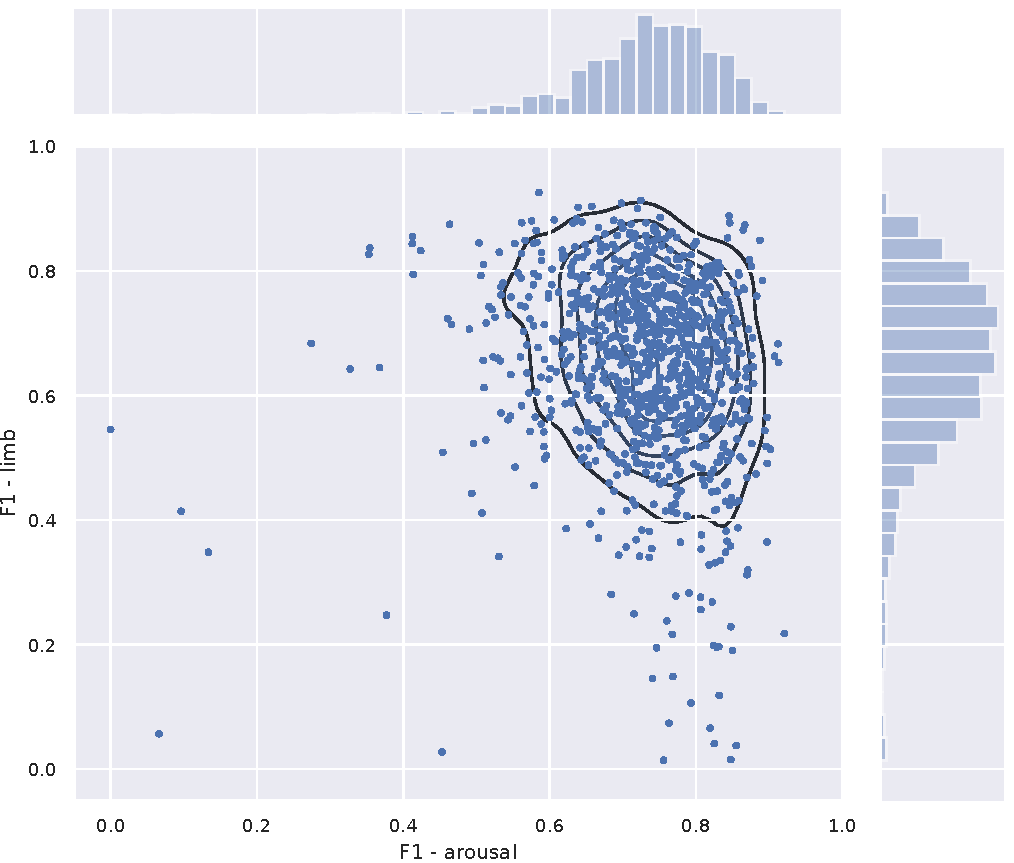
\includegraphics[width=\textwidth]{figures/paper-iv/embc19-distribution.pdf}
    \caption[Visualization of F1 scores]{Visualization of F1 scores for both \ac{Ar} and \ac{LM} detection using the dynamic model.}
    \label{fig:paperiv-test_distribution}
\end{figure}
\begin{table}[tb]
    \sisetup{separate-uncertainty}
    \small
    \centering
    \begin{threeparttable}
    \caption[Optimized test performance]{Application of optimized models on \test data.}
    \label{tab:paperiv-test_results}
    \begin{tabular}{@{}lSSS@{}} \toprule
        \textbf{Model} & \textbf{F1} & \textbf{Pr} & \textbf{Re} \\ \midrule
        \ac{LM}, static & \num{0.648 \pm 0.148} & \num{0.631 \pm 0.181} & \num{0.720 \pm 0.141} \\
        \ac{Ar}, static & \num{0.727 \pm 0.102} & \num{0.706 \pm 0.113} & \num{0.771 \pm 0.132} \\
        \ac{LM}, dynamic & \num{0.647 \pm 0.148} & \num{0.627 \pm 0.181} & \num{0.722 \pm 0.14} \\
        \ac{Ar}, dynamic. & \num{0.729 \pm 0.102} & \num{0.699 \pm 0.115} & \num{0.785 \pm 0.131} \\ \midrule
        \ac{LM}, \ac{RNN} & \num{0.639 \pm 0.147} & \num{0.606 \pm 0.180} & \num{0.727 \pm 0.126} \\
        \ac{Ar}, \ac{RNN} & \num{0.749 \pm 0.105} & \num{0.772 \pm 0.107} & \num{0.748 \pm 0.138} \\ \bottomrule
    \end{tabular}
    \begin{tablenotes}
    \item Data are shown as subject-averaged F1, precision (Pr) and recall (Re) with associated standard deviations. Top four rows correspond to Experiment A, while bottom two rows correspond to Experiment B. \ac{Ar}: arousal; \ac{LM}: leg movement; \ac{RNN}: recurrent neural network.
    \end{tablenotes}
    \end{threeparttable}
\end{table}
In this work, we investigated somatic \ac{PSG} events present in multiple signal modalities instead of \ac{EEG}-specific events, which required changes to the network architecture. 
Specifically, we kept the signal modality encoded in the first dimension of the tensor propagated through the network, which allowed for the use of \oned convolutional operators. 
By performing \oned convolutions and keeping the channel information in the feature maps instead of keeping them as separate dimensions and performing \twod convolutions as proposed in~\cite{Chambon2018b,Chambon2019}, we simplify and reduce the number of computations and training time by a factor $\propto C$. 

However, we did not investigate the effects of modeling the conditional probability of \ac{Ar} and \ac{LM} occurrence, but the proposed architecture is versatile enough to detect both events jointly as well as separately. 
Previous work also suggest that detecting multiple objects at the same time is of high interest and leads to (at least) non-inferior performances~\cite{Chambon2018b, Chambon2019, Redmon2016a, Redmon2016b, Liu2016}.

Additionally, we speculated that the temporal dynamics of the \ac{PSG} signals were important for optimal event detection performance. 
Although the effects were small, the F1 score in \ac{Ar} detection increased when adding an \ac{RNN} module to the network before the detection module. 
However, this was not the case for \ac{LM} detection, which is most likely due to the different temporal and physiological characteristics of the two events in question. 

Future efforts will address the fact that events are mutually exclusive in the current modeling scheme, given a certain default event window size. 
However, it is common to see \acp{Ar} and \acp{LM} as a result of one another, and thus, if the window size is too small, a more unlikely event, as measured by classification threshold and \ac{IoU}, will be removed even if it matches up to a specific true event of a certain class. 
\section{Paper V: Deep transfer learning for improving single-EEG arousal detection}\label{sec:paperv}
\sectionmark{Olesen, Jennum, Mignot, \& Sorensen, 2020}

\subsection{Methods}

\paragraph*{Notation} We denote by \(\llbracket a, b \rrbracket\) the set of integers \(\lbrace n \in \N \mid a \leq n \leq b\rbrace\) with \(\llbracket N \rrbracket\) being shorthand for \(\llbracket 1, N \rrbracket\), and by \(n \in \llbracket N \rrbracket \) the \(n\)th sample in \(\llbracket N \rrbracket\).
A model for a given experiment is denoted by $\mathcal{M}_{(\cdot)}$, while an optimized model is superscripted with a star as $\mathcal{M}_{(\cdot)}^{*}$.
A segment of PSG data is denoted by $\mathbf{x} \in \real^{C \times T}$, where $C, T$ is the number of channels and the duration of the segment in samples, respectively.

\subsubsection{Data}
We collected PSGs from \num{1500} subjects in the MrOS Sleep Study~\cite{Blank2005, Orwoll2005, Blackwell2011} from the National Sleep Research Resource repository~\cite{Dean2016, Zhang2018}.
From each PSG, we extracted left and right EEG, left and right EOG, and chin EMG.
EEG and EOG channels were referenced to the contralateral mastoid process.
For each PSG, we also extracted time-stamped arousal scorings containing starts and durations of scored arousal events.
We did not exclude any PSGs from this study based on sleep duration, number of arousal events, or similar criteria.

\subsubsection{Data partitioning}
The 1500 PSGs were initially partitioned into three subsets \train\textsubscript{1}, \eval\textsubscript{1}, and \test\textsubscript{1} containing 400, 100 and 1000 PSGs, respectively.
Furthermore, we additionally partitioned \test\textsubscript{1} into three smaller subsets \train\textsubscript{2}, \eval\textsubscript{2}, and \test\textsubscript{2} containing 400, 100, and 500 PSGs, respectively.

\subsubsection{Preprocessing pipeline}
All signals were resampled to \SI{128}{\hertz} using poly-phase filtering with a Kaiser window ($\beta = 5.0$) prior to subsequent processing.
Extracted EEG and EOG signals were filtered with \nth{2} order Butterworth IIR bandpass filters with cutoff frequencies \SI{0.3}{\hertz} and \SI{35}{\hertz}. 
Chin EMG was filtered with a \nth{4} order Butterworth IIR highpass filter with a cutoff frequency of \SI{10}{\hertz}.
Filtered signals were subsequently standardized by 
\begin{equation}
    \mathbf{x}^{(i)} = \frac{\tilde{\mathbf{x}}^{(i)} - \boldsymbol{\mu}^{(i)}}{\boldsymbol{\sigma}^{(i)}},
\end{equation}
where $\tilde{\mathbf{x}}^{(i)} \in \real^{C \times T}$ is the raw matrix containing $C$ input channels and $T$ samples, and $\boldsymbol{\mu}^{(i)}, \boldsymbol{\sigma}^{(i)} \in \real^{C}$ are the mean and standard deviation vectors for the \textit{i}'th PSG, respectively.

\subsubsection{Model setup}
We expand upon previous work using similar models for sleep event detection~\cite{Chambon2018b, Chambon2019, Olesen2019}. 
Briefly, the model takes as input a tensor of PSG data $\mathbf{x} \in \real^{C \times T}$ and outputs 
\begin{equation}
    \mathbf{z} = \left( \mathbf{p}, \mathbf{y} \right) \in \real^{N_d \times T^{\prime} \times (K+1)} \times \real^{N_d \times T^{\prime} \times 2}
\end{equation}
containing predicted arousal probabilities $\mathbf{p}$ and associated start and durations for predicted arousal events $\mathbf{y}$.
The differentiable function underlying the model comprises a deep neural network architecture consisting of the following modules:
\paragraph{Input mixing module}
Here, non-linear combinations of the input PSG data $\mathbf{x}$ are made using a non-linear mixing block $\phi_{\mathrm{mix}} : \real^{1 \times C \times T} \to \real^{C \times 1 \times T}$.
\paragraph{Feature extraction module}
This module contains two components. 
The first is a convolutional feature extraction block $\varphi_{\mathrm{conv}} : \real^{C \times 1 \times T} \to \real^{f^{\prime} \times 1 \times T^{\prime}}$ consisting of $k_{\mathrm{max}}$ successions of convolutional, batch normalization, and rectified linear unit (ReLU) layers.
Second is a recurrent feature extraction block $\varphi_{\mathrm{rec}} : \real^{f^{\prime} \times 1 \times T^{\prime}} \to \real^{f^{\prime} \times 2 \times T^{\prime}}$ with $f^{\prime}=f_02^{k_{\mathrm{max}}}$ hidden units.
The $\varphi_{\mathrm{conv}}$ block is responsible for bulk feature extraction and temporal decimation using strided convolutions, while $\varphi_{\mathrm{rec}}$ processes the raw features across the reduced temporal dimension using a bidirectional gated recurrent unit~\cite{Cho2014} with $f^{\prime}$ hidden units.
\paragraph{Event detection module}
The output from $\varphi_{\mathrm{rec}}$ is processed by two separate blocks: $ \psi_{\mathrm{clf}} : \real^{f^{\prime} \times 2 \times T^{\prime}} \to \real^{\left( K + 1 \right) \! N_d \times 1 \times T^{\prime}} $ outputs the tensor $\mathbf{p}$ containing predicted arousal probabilities for each time point $t \in \llbracket T^{\prime} \rrbracket$ for each default event window. 
$ \psi_{\mathrm{loc}} : \real^{f^{\prime} \times 2 \times T^{\prime}} \to \real^{2N_d \times T^{\prime}} $ outputs the tensor $\mathbf{y}$ containing predicted start time and durations of arousal events. 
Both $\psi_{\mathrm{clf}}$ and $\psi_{\mathrm{loc}}$ are implemented using $\left(2, 1\right)$ convolutions rather than convolutions over the entire volume as in~\cite{Chambon2018b, Chambon2019, Olesen2019}.
This serves a dual purpose: the first is to reduce the number of parameters to make the network more memory-efficient, while the second purpose is to allow the kernel and feature maps to be temporally invariant.

For a detailed description of the network architecture, see~\cref{tab:paperv-architecture}.

\begin{landscape}
\begin{table}[tb]
    \begin{threeparttable}
        \centering
        \caption[MSED architecture overview]{Network architecture overview.} 
        \label{tab:paperv-architecture}
        \begin{tabular}{@{}llllllll@{}}
            \toprule
            \textbf{Module} & \textbf{Layer type} & \textbf{Kernel} & \textbf{Stride} & \textbf{Feature maps} & \textbf{Input size} & \textbf{Output size} & \textbf{Activation} \\ \midrule
            \(\mathbf{x}\) & Input & --- & --- & --- & \( C \times T \) & \( 1 \times C \times T \) & --- \\
            \( \phi_{\mathrm{mix}} \) & 2D convolution & \( (C, 1) \) & \( (1, 1) \) & \( C \) & \( 1 \times C \times T \) & \( C \times 1 \times T \) & ReLU \\ \midrule
            \( \varphi_{\mathrm{conv},1} \) & 2D convolution & \( (1, c) \) & \( (1, s) \) & \( 2f_0 \) & \( C \times 1 \times T \) & \( 2f_0 \times 1 \times T/s \) & --- \\
            & Batch norm. & --- & --- & \(2f_0\) & \(2f_0 \times 1 \times T/s\) & \(2f_0 \times 1 \times T/s\) & ReLU \\
            \( \varphi_{\mathrm{conv},k} \) & 2D convolution & \( (1, c) \) & \( (1, s) \) & \( f_02^{k} \) & \( f_02^{k-1} \times 1 \times T/s^{k-1} \) & \( f_02^{k} \times 1 \times T/s^k \) & --- \\
            \( k \in \llbracket 2, k_{\mathrm{max}} \rrbracket \) & Batch norm. & --- & --- & \(f_02^{k}\) & \(f_02^{k} \times 1 \times T/s^k\) & \(f_02^{k} \times 1 \times T/s^k\) & ReLU \\
            \( \varphi_{\mathrm{rec}} \) & bGRU & --- & --- & $f^{\prime}$ & \( f^{\prime} \times 1 \times T^{\prime} \) & \( f^{\prime} \times 2 \times T^{\prime} \) & --- \\ \midrule
            \( \psi_{\mathrm{clf}} \) & 2D convolution & \( (2, 1) \) & \( (1, 1) \) & \( \left( K + 1 \right) \! N_d \) & $f^{\prime} \times 2 \times T^{\prime}$ & $\left( K + 1 \right) \! N_d \times 1 \times T^{\prime}$ & Softmax over \( K + 1 \) \\
            \( \psi_{\mathrm{loc}} \) & 2D convolution & \( (2, 1) \) & \( (1, 1) \) & \( 2 N_d \) & $f^{\prime} \times 2 \times T^{\prime}$ & $2 N_d \times 1 \times T^{\prime}$ & Linear \\ \midrule
            \(\mathbf{z}\) & Output, \(\mathbf{p}\) & --- & --- & --- & $\left( K + 1 \right) \! N_d \times 1 \times T^{\prime}$ & $N_d \times T^{\prime} \times \left( K + 1 \right)$ & --- \\
             & Output, \(\mathbf{y}\) & --- & --- & --- & $2 N_d \times 1 \times T^{\prime}$ & $N_d \times T^{\prime} \times 2$ & --- \\
            \bottomrule
        \end{tabular}
        \begin{tablenotes}
            \small
            \item \(\mathbf{x}\), input containing PSG data; $\mathbf{z}$, output containing predicted arousal probabilities and associated start and duration predictions; \( \phi_{\mathrm{mix}} \), non-linear mixing block; \(\varphi_{\mathrm{conv}}\), convolutional feature extraction block; \( \varphi_{\mathrm{rec}} \) recurrent feature extraction block; \( \psi_{\mathrm{clf}} \), event classification block; \( \psi_{\mathrm{loc}} \), event localization block; $C$, number of input channels; $T$, number of samples in a segment of PSG data; $c$, temporal kernel size; $s$, temporal stride; $f_0$, base number of feature maps; $f^{\prime}=f_02^{k_{\mathrm{max}}}$, maximum number of feature maps; $T^{\prime} = T/s^{k_{\mathrm{max}}}$, reduced temporal dimension in samples; $N_d$, number of default event windows in segment; $K$, number of classes; ReLU, rectified linear unit; bGRU, bidirectional gated recurrent unit.
        \end{tablenotes}
    \end{threeparttable}
\end{table}
\end{landscape}

\subsubsection{Loss objective}
The network parameters were optimized according to a three-component loss objective comprising a localization loss \( \ell_{\mathrm{loc}} \) and a positive and negative classification loss $\ell_{+}$ and $\ell_{-}$, respectively, such that
\begin{equation}\label{eq:paperv-loss}
    \ell = \ell_{\mathrm{loc}} + \ell_{+} + \ell_{-}.
\end{equation}
The localization loss was calculated using a Huber function
\begin{equation}
    \ell_{\mathrm{loc}} = \frac{1}{N_{\pi \backslash \emptyset}} \sum_{i \in \pi \backslash \emptyset}\!{h^{(i)}} \\
    % \ell_{\mathrm{loc}} = \frac{1}{\sum_{i}{i \\pi \backslash \emptyset}} \sum_{i \in \pi \backslash \emptyset}\!{h^{(i)}} \\
\end{equation} 
\begin{equation}
    \mathbf{h} =
    \begin{cases}
        0.5 \! \left( \mathbf{y} - \mathbf{t} \right)^2, & \text{if } \lvert \mathbf{y} - \mathbf{t} \rvert < 1, \\
        \lvert \mathbf{y} - \mathbf{t} \rvert - 0.5, & \text{otherwise,}
    \end{cases}
\end{equation}
where $i \in \pi \backslash \emptyset$ indicates event windows with a non-empty arousal target.
Contributions from the positive/negative classification losses were calculated using a focal loss function~\cite{Lin2020}:
\begin{align}
    \ell_{+} &= \frac{1}{N_{\pi \backslash \emptyset}} \sum_{i \in \pi \backslash \emptyset}\!{-\alpha \left( 1 - \mathbf{p} \right)^{\gamma}\log \left( \mathbf{p} \right)}, \, \text{and} \\
    \ell_{-} &= \frac{1}{N_{\pi = \emptyset}} \sum_{i \in \pi = \emptyset}\!{-\alpha \left( 1 - \mathbf{p} \right)^{\gamma}\log \left( \mathbf{p} \right)},
\end{align}
where $\alpha=0.25$ and $\gamma=2$.
This serves to counter the class imbalance in a single data segment, which typically consists of many event windows with few positive examples.

\subsubsection{Experimental setups}
We investigated the channel mismatch problem with the following four experimental setups:
\paragraph{Full montage baseline (FM)}
In this experiment, we trained the event detection algorithm on $\train_1$ using \(C=5\) channels: left/right central EEG, left/right EOG, and chin EMG.
Convergence and the optimal detection threshold were assessed on $\eval_1$ and performance was evaluated on \test\textsubscript{2}.
The optimal baseline model was used as an initialization for the two transfer learning experiments described below.
\paragraph{Pretraining (PT)}
The optimal model $\mbl^{*}$ was used in this experiment as an initialization for $\mpt$.
We adjusted the mixing module and first convolutional layer in the feature extraction module to account for the channel mismatch by replacing the convolutional and batch normalization layers, and subsequently trained these from scratch.
The rest of the weights and bias terms were frozen to the optimized values from $\mbl^{*}$.
The network was trained on $\train_2$ with only $C=1$ channels (left central EEG, C3).
Convergence and optimal detection threshold were assesed on $\eval_2$, while final performance was evaluated on \test\textsubscript{2}.
\paragraph{Fine-tuning (FT)}
Similar to PT, the optimal model $\mbl^{*}$ was used in this experiment as an initialization for $\mft$.
Also, the mixing module and first convolutional layer in the feature extraction module were likewise adjusted.
However, all other layers in $\mft$ were permitted to be further optmized by fine-tuning weights and bias terms during training.
The model was trained using the same 400 PSGs from $\train_2$ with the same $C=1$ channel configuration as in PT.
\paragraph{Single EEG benchmark (SE)}
We benchmarked our two transfer learning experiments to a comparable situation in which an event detection model was trained on the same PSGs in $\train_2$ using only the left central EEG (C3).



In all experimental runs, we optimized the loss objective in~\cref{eq:paperv-loss} using the Adam optimization algorithm with a learning rate of \(\alpha=10^{-3}\) and the default parameter values \( \left( \beta_1, \beta_2 \right) = \left( 0.9, 0.999 \right) \) as suggested in~\cite{Kingma2015}.
We applied the same data sampling strategy as proposed in~\cite{Olesen2019}, in which a segment of data is sampled such that it contains at least 50\% of a randomly sampled event across all PSGs.
We used a default event window size of \SI{15}{\second} with \SI{50}{\percent} overlap as this was found previously to work well for arousal detection~\cite{Olesen2019}.

All experiments were implemented in PyTorch 1.2~\cite{Paszke2019}.

\subsubsection{Performance evaluation}
Bipartite matching were used to match detected and true events during training and testing.
At test time, detected events were subjected to non-maximum suppression based on an intersection-over-union (IOU) of at least 0.5 between detected and true events.
We evaluated the performance of our experimental setups using precision, recall and F1 scores.

\subsubsection{Statistical analysis}
We used Kruskal–Wallis one-way analysis of variance tests for differences in performance metrics between groups (SE, FT and PT) with a significance level of $\alpha=0.05$.
Post-hoc testing was performed with Mann-Whitney U-tests for each pair-combination (SE/FT, SE/PT, and FT/PT) likewise with $\alpha=0.05$.
We accounted for multiple comparisons by adjusting \textit{p}-values with Bonferroni corrections.


\subsection{Results}
\begin{figure}[tb]
    \centering
    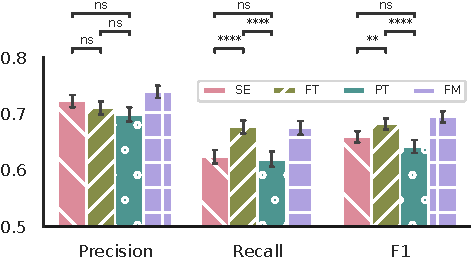
\includegraphics[width=\columnwidth]{figures/paper-v/paperv-figure01.pdf}
    \caption[MSED-TL performance on \test\textsubscript{2}]{Performance metrics as evaluated on \test\textsubscript{2} for each experimental setup. Metrics are shown as means with 95\% confidence interval as error bars. Note the $y$-axis scaling. SE: single-EEG. FT: fine-tuning. PT: pre-training. FM: full montage. ns: not significant, $^{**}$: $p_{\mathrm{adj}} \leq 10^{-2}$; $^{****}$: $p_{\mathrm{adj}} \leq 10^{-4}$.}
    \label{fig:paperv-figure01}
\end{figure}

\begin{table}[tb]
    \centering
    \begin{threeparttable}
        \footnotesize
        \caption{Performance metrics across experiments.}
        \label{tab:paperv-results}
        \begin{tabular}{@{}lccc@{}}
        \toprule
        \textbf{Experiment} &        \textbf{Precision} &           \textbf{Recall} &               \textbf{F1} \\ \midrule
        FM &  $0.739 \pm 0.122$ &  $0.675 \pm 0.139$ &  $0.694 \pm 0.115$ \\
        SE &  $0.723 \pm 0.124$ &  $0.624 \pm 0.137$ &  $0.659 \pm 0.117$ \\ \midrule
        FT &  $\mathbf{0.710 \pm 0.128}$ &  $\mathbf{0.676 \pm 0.130}$ & $\mathbf{0.682 \pm 0.110}$ \\
        PT &  $0.699 \pm 0.141$ &  $0.619 \pm 0.153$ &  $0.642 \pm 0.129$ \\
        \bottomrule
        \end{tabular}
        \begin{tablenotes}
            \small
            \item Metrics are shown evaluated on \test\textsubscript{2} as means $\pm$ standard deviation. Best performing transfer learning experiment is shown in bold. SE: single-EEG. FT: fine-tuning. PT: pre-training. FM: full montage.
        \end{tablenotes}
    \end{threeparttable}
\end{table}

We show the results of the transfer learning experiments (FT, PT) as well as the baseline and benchmark experiments (FM, SE) in~\cref{fig:paperv-figure01} and~\cref{tab:paperv-results}. 
Performance metrics were not calculated for \num{10} subjects in \test\textsubscript{2}, as these did not have any scored arousals and are thus not reflected in~\cref{fig:paperv-figure01} and~\cref{tab:paperv-results}.

The baseline F1 performance is shown to be slightly lower than previously reported ($0.694 \pm 0.115$ vs. $0.749 \pm 0.105$~\cite{Olesen2019}).
However, our baseline model was trained on \num{400} subjects compared to \num{1485} in~\cite{Olesen2019}, which would account for the lower F1 score. 
By reducing the available input channels from $C=5$ different modalities to $C=1$ EEG channels as in the SE benchmark experiment, the F1 score drops to $0.659 \pm 0.117$, while the precision and recall scores likewise drop from $0.739 \pm 0.122$ to $0.723 \pm 0.124$, and $0.675 \pm 0.139$ to $0.624 \pm 0.137$, respectively.

We found statistically significant differences in F1 scores between SE, FT, and PT ($p=3.189\times 10^{-7}$). 
Post-hoc testing further revealed statistically significant differences between SE and FT ($p_{\mathrm{adj}}=2.224 \times 10^{-3}$), and FT and PT ($p_{\mathrm{adj}}=2.685 \times 10^{-7}$), but not between SE and PT  ($p_{\mathrm{adj}}=0.080$). 
We also found that recall scores differed between experimental setups ($p=7.085 \times 10^{-13}$).
Post-hoc testing showed statistically significant differences between SE, FT ($p_{\mathrm{adj}}=5.180 \times 10^{-11}$), and FT and PT ($p_{\mathrm{adj}}=1.440 \times 10^{-9}$), but not between SE and PT ($p_{\mathrm{adj}}=1.000$).
Lastly, we saw statistically significant differences in precision scores between experimental setups ($p=0.033$), subsequent post-hoc testing did not reveal any statistical significant differences, when adjusting for multiple comparisons using the Bonferroni procedure (SE/FT, $p_{\mathrm{adj}}=0.214$; FT/PT, $p_{\mathrm{adj}}=1.000$; SE/PT, $p_{\mathrm{adj}}=0.037$).

Our results show, that for some scenarios, we can learn information present in multi-variate PSG data and efficitively transfer that information to a target domain containing only a single EEG channel.
Specifically, the performance of our fine-tuning strategy is high enough that the mean F1 scores across subjects are statistically insifignicant, when comparing FT and FM setups (not shown).

Previous related work focused on the channel mismatch problem, when comparing different, but the same number of, channel modalities such as transferring EEG-based models to EOG-based target domains, and thus did not investigate how changing the model architecture might impact performance~\cite{Phan2019, Phan2019c}.
In this work, we investigated transfer learning when the source and target domains only overlap by one input channel.
This necessitates changing some parts of the underlying model architecture to accommodate the different number of input channels, and these changes might impact downstream feature extraction.
We did not explore simply zeroing out a large number of input channels in this work, as this requires exhaustive search of which channel indices to zero out in the model based on the number of target input channels. 
Our strategy does not require this exhaustive search.

Our study applied a simple optimization strategy for the transfer learning experiments, which might limit the potential performance gain.
This is especially relevant for the FT experiment. 
For example, one could experiment with with different learning rates and scheduling schemes for the initial layers and pre-trained layers, such that the initial layers were trained with a higher relative learning rate to compensate for their lack of initial training.

Furthermore, we explored transfer learning for the channel mismatch problem in a single cohort of patient recordings. 
Future directions of this research will investigate scenarios, where both the source and target domains, and the datasets are different.
% \section{Paper VI: Olesen, \textit{et al.}, 2020c}
\subsection{Methods}
\subsection{Results}


\section{Chapter summary}\label{sec:eventdetection-summary}

Aspects that were not investigated in this thesis, but are of interest in future work include
\begin{itemize}
    \item An evaluation of individual sleep events when placed in the context of a micro-sleep architecture, \eg a high-resolution hypnodensity.
\end{itemize}